\documentclass[12pt]{article}
\usepackage{lmodern}
\usepackage[T1]{fontenc}
\usepackage[portuges]{babel}
\usepackage[utf8]{inputenc}
\usepackage{a4}
\usepackage{textgreek}
\usepackage{epstopdf}
\usepackage{graphicx}
\usepackage{fancyvrb}
\usepackage{amsmath}
\usepackage{float}
\usepackage{listings}
%\renewcommand{\baselinestretch}{1.5}


\begin{document}

\begin{titlepage}

\newcommand{\HRule}{\rule{\linewidth}{0.5mm}} % Defines a new command for the horizontal lines, change thickness here

\center % Center everything on the page
    
%----------------------------------------------------------------------------------------
%	HEADING SECTIONS
%----------------------------------------------------------------------------------------

\textsc{\LARGE Universidade do Minho}\\[1.5cm] 
\textsc{\Large Mestrado Integrado em Engenharia Informática}\\[0.5cm] 
\textsc{\large Computação Gráfica}\\[0.5cm]

%----------------------------------------------------------------------------------------
%	TITLE SECTION
%----------------------------------------------------------------------------------------

\HRule \\[0.4cm]
{ \huge \bfseries Primitivas Gráficas}\\[0.4cm] 
\HRule \\[1.5cm]
    
%----------------------------------------------------------------------------------------
%	AUTHOR SECTION
%----------------------------------------------------------------------------------------

\begin{minipage}{0.4\textwidth}
\begin{flushleft} \large
\emph{Grupo:}\\
Etienne Costa A76089 \\
Joana Cruz A76270 \\
Rafael Alves A72629 \\
Maurício Salgado A71407 \\
\end{flushleft}
\end{minipage}
~
\begin{minipage}{0.4\textwidth}
\begin{flushright} \large
\emph{Docente:} \\
António Ramires\\
\end{flushright}
\end{minipage}\\[2cm]

%----------------------------------------------------------------------------------------
%	DATE SECTION
%----------------------------------------------------------------------------------------

{\large \today}\\[2cm]

%----------------------------------------------------------------------------------------
%	LOGO SECTION
%----------------------------------------------------------------------------------------


\includegraphics[scale=0.3]{uminho}\\
    
%----------------------------------------------------------------------------------------

\vfill % Fill the rest of the page with whitespace

\end{titlepage}
\tableofcontents
\newpage
\section{Introdução}
O relátorio apresentado diz respeito à primeira fase do trabalho proposto no âmbito da unidade curricular de Computação Gráfica. O trabalho
consiste no desenvolvimento de um gerador de vértices de algumas primitivas gráficas sendo estas um plano, uma caixa, uma esfera e um cone). Para além disto, também foi desenvolvida
uma aplicação de leitura de ficheiros de configuração em XML(Engine) que servirá para desenhar os vértices anteriormente gerados. Para o desenvolvimento deste projeto foi
necessário utilizar certos recursos como a linguagem C++ e o OpenGL.
\newpage
\section{Gerador}
Esta aplicação tem como objetivo gerar todos os vértices necessários para a elaboração dos triângulos que constituem a figura pretendida e guardar num ficheiro.
A função main do gerador vê qual a primitiva gráfica que se pretende gerar, como já referimos, pode ser um plano, uma caixa, uma esfera ou um cone.
De seguida chama a função geradora correspondente, tendo em conta o número de argumentos pedidos, e escreve como resultado os vértices gerados.\newline
\begin{center}
\fbox{\begin{minipage}{25em}
Generator.exe <modelo> [parâmetros] <outputFile>
\end{minipage}}
\end{center}
\begin{itemize}
\item\textbf{Plano} - apenas recebe um argumento, por ser pedido um plano quadrado e corresponde ao lado do plano. 
\item\textbf{Caixa} - recebe como argumentos o comprimento, a altura, a largura e o número de divisões. Caso não se pretenda dividir este último argumento tomará o valor 1.
\item\textbf{Esfera} - recebe como argumentos o raio, o número de slices(divisões verticais) e o número de stacks(divisões horizontais).
\item\textbf{Cone} - recebe os mesmos argumentos da esfera, incluindo a altura do cone.
\end{itemize}
\newpage
\section{Plano}
É pretendido um plano $XZ$ quadrado, centrado na origem e obtido com 2 triângulos. 
Para calcular os pontos que constituem o plano precisamos do tamanho que nos dará informação sobre a dimensão do plano
no eixo dos $xx$, e dimensão do plano no eixo dos $zz$. 
O plano contém 4 pontos e sendo centrado na origem temos que efetuar os seguintes cálculos: \newline
\begin{center}
$x = tamanho/2$ \newline
$y = 0$ \newline
$z = tamanho/2$ \newline
\end{center}
\begin{figure}[H]
\centering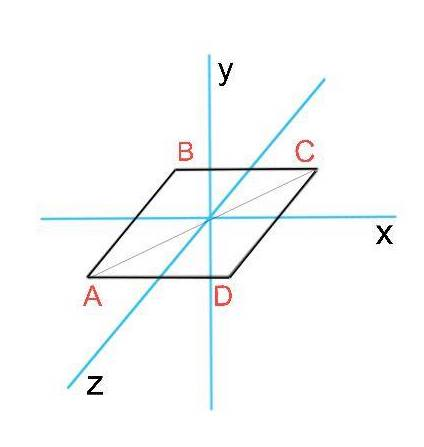
\includegraphics[scale=0.4]{planoXZ} 
\caption{\label{fig:controller}Figura ilustrativa de um plano XZ}
\end{figure} 
Efetuando os cálculos, obtemos os seguintes pontos: \newline
\begin{center}
$A = (-x,y,z)$ \newline 
$B = (-x,y,-z)$ \newline 
$C = (x,y,-z)$ \newline 
$D = (x,y,z)$ \newline
\end{center}
Gerando o plano a partir do ponto A, e segundo o openGL, para a superfície do plano ficar visível utilizamos a regra da mão direita no sentido inverso aos ponteiros do relógio,
obtemos que os vértices dos triângulos $ACB$ e $ADC$, terão como coordenadas: \newline
\begin{center}
$ACB\rightarrow (-x,y,z) (x,y,-z) (-x,y,-z) $ \newline
$ADC\rightarrow (-x,y,z) (x,y,z) (x,y,-z)$ \newline
\end{center}
Exemplo: \textit{plane 5}
\begin{figure}[H]
\centering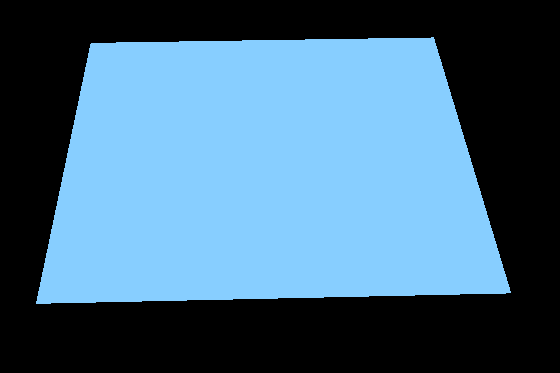
\includegraphics[scale=0.45]{planoP} 
\caption{\label{fig:controller}Exemplo de um plano}
\end{figure} \begin{figure}[H]
\centering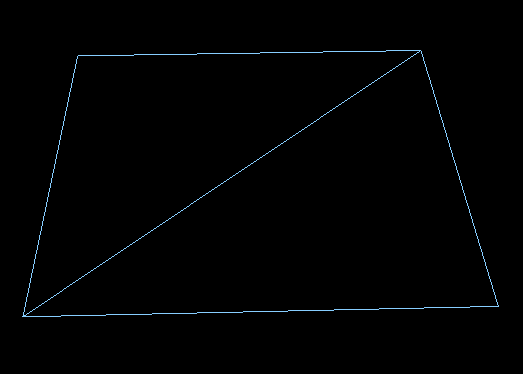
\includegraphics[scale=0.45]{planoT} 
\caption{\label{fig:controller}Exemplo de um plano com a representação dos triângulos}
\end{figure} 
Caso fosse pedido qualquer plano $XZ$ teríamos que receber dois parâmetros: as dimensões do plano no eixo do xx e no eixo zz. 
\newpage
\section{Caixa}
O cálculo dos pontos de uma caixa precisa dos seguintes parâmetros: \textit{comprimento}(dimensão no eixo dos $xx$),
\textit{altura}(dimensão no eixo dos $yy$), \textit{largura}(dimensão no eixo dos $zz$) e o número de \textit{divisões}. 
Uma caixa pode ou não conter divisões pelo que precisamos de guardar informação sobre o número de divisões, sendo estas calculadas pelas seguintes equações:
\begin{center}
$divX = \frac{dimX}{div}$ \newline\newline
$divY = \frac{dimY}{div}$ \newline\newline
$divZ = \frac{dimZ}{div}$ \newline\newline
\end{center}
E de modo a que a caixa fique centrada na origem precisamos das coordenadas $x,y$, e $z$ do seu centro:
\begin{center}
$dimX = \frac{comprimento}{2}$ \newline\newline
$dimY = \frac{altura}{2}$ \newline\newline
$dimZ = \frac{largura}{2}$ \newline\newline
\end{center}
Necessitamos de calcular todos os vértices que constituem a caixa, que é constítuida por 6 faces. Primeiramente, calculamos as faces XZ, 
de seguida as faces XY e por último as faces YZ. Todas estas fases seguem o mesmo processo: calcula-se os seis vértices pertencentes aos dois triângulos
de uma divisão, usamos a regra da mão direita no sentido contrário aos ponteiros do relógio nas faces visíveis para nós, enquanto
as faces opostas são calculadas no sentido dos ponteiros do relógio. O posicionamento inicial é sempre a origem e este processo é repetido quantas vezes o número de divisões.\newline\newline
\subsection{Cálculo das faces XZ}
\begin{figure}[H]
\centering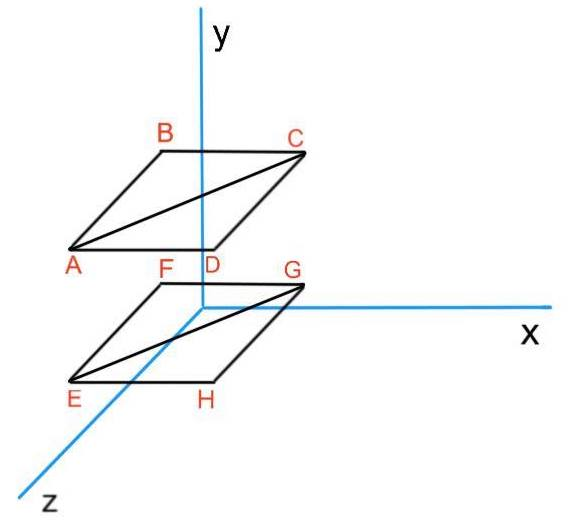
\includegraphics[scale=0.45]{XZ} 
\caption{\label{fig:controller}Faces XZ de uma caixa sem divisões}
\end{figure}
\textbf{Para $ i = 0$ até div fazer $i++\{$} \newline
\par $x = i\times divX$\newline
\par \textbf{Para $ j = 0$ até div fazer $j++\{$} \newline
\par $z = j\times divZ$\newline
\par\textit{\textbf{Cálculo da face de cima - Triângulos ACB e ADC}} \newline
\par$xa = x - dimX$ \newline
\par$ya = dimY$ \newline
\par$za = z-dimZ+divZ$ \newline\newline
\par$xb = x - dimX$ \newline
\par$yb = dimY$ \newline
\par$zb = z - dimZ$ \newline\newline
\par$xc = x - dimX + divX$ \newline
\par$yc = dimY$ \newline
\par$zc = z - dimZ$ \newline\newline
\par$xd = x - dimX + divX$ \newline
\par$yd = dimY$ \newline
\par$zd = z - dimZ + divZ$ \newline\newline
\par\textit{\textbf{Cálculo da face de baixo - Triângulos EFG e EGH}} \newline
\par$xe = x - dimX$ \newline
\par$ye = -dimY$ \newline
\par$ze = z-dimZ+divZ$ \newline\newline
\par$xf = x - dimX$ \newline
\par$yf = -dimY$ \newline
\par$zf = z - dimZ$ \newline\newline
\par$xf = x - dimX + divX$ \newline
\par$yg = -dimY$ \newline
\par$zg = z - dimZ$ \newline\newline
\par$xh = x - dimX + divX$ \newline
\par$yh = -dimY$ \newline
\par$zh = z - dimZ + divZ$ \newline\newline
\par $\}$ \newline
$\}$\newline\newline
\subsection{Cálculo das faces XY}
\begin{figure}[H]
\centering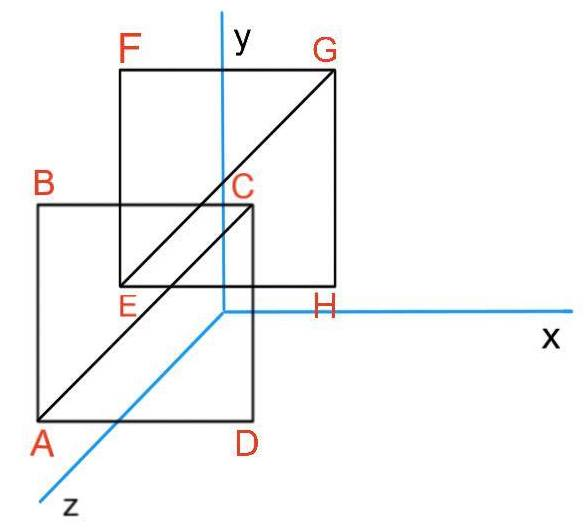
\includegraphics[scale=0.45]{XY} 
\caption{\label{fig:controller}Faces XY de uma caixa sem divisões}
\end{figure}
\textbf{Para $ i = 0$ até div fazer $i++\{$} \newline
\par $x = i\times divX$\newline
\par \textbf{Para $ j = 0$ até div fazer $j++\{$} \newline
\par $y = j\times divY$\newline
\par\textit{\textbf{Cálculo da face da frente - Triângulos ACB e ADC}} \newline
\par$xa = x - dimX$ \newline
\par$ya = y-dimY$ \newline
\par$za = dimZ$ \newline\newline
\par$xb = x - dimX$ \newline
\par$yb = y - dimY + divY$ \newline
\par$zb = dimZ$ \newline\newline
\par$xc = x - dimX + divX$ \newline
\par$yc = y - dimY + divY$ \newline
\par$zc = dimZ$ \newline\newline
\par$xd = x - dimX + divX$ \newline
\par$yd = y - dimY$ \newline
\par$zd = dimZ$ \newline\newline
\par\textit{\textbf{Cálculo da face de trás - Triângulos EFG e EGH}} \newline
\par$xe = x - dimX$ \newline
\par$ye = y-dimY$ \newline
\par$ze = -dimZ$ \newline\newline
\par$xf = x - dimX$ \newline
\par$yf = y - dimY + divY$ \newline
\par$zf = -dimZ$ \newline\newline
\par$xg = x - dimX + divX$ \newline
\par$yg = y - dimY + divY$ \newline
\par$zg = -dimZ$ \newline\newline
\par$xh = x - dimX + divX$ \newline
\par$yh = y - dimY$ \newline
\par$zh = -dimZ$ \newline\newline
\par $\}$ \newline
$\}$\newline\newline
\subsection{Cálculo das faces YZ}
\begin{figure}[H]
\centering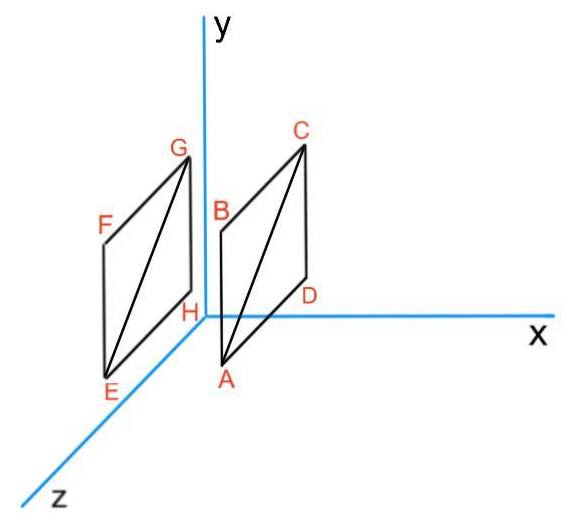
\includegraphics[scale=0.45]{YZ} 
\caption{\label{fig:controller}Faces YZ de uma caixa sem divisões}
\end{figure}
\textbf{Para $ i = 0$ até div fazer $i++\{$} \newline
\par $y = i\times divY$\newline
\par \textbf{Para $ j = 0$ até div fazer $j++\{$} \newline
\par $z = j\times divZ$\newline
\par\textit{\textbf{Cálculo da face lateral direita - Triângulos ACB e ADC}} \newline
\par$xa = dimX$ \newline
\par$ya = y - dimY$ \newline
\par$za = z-dimZ+divZ$ \newline\newline
\par$xb = dimX$ \newline
\par$yb = y - dimY + divY$ \newline
\par$zb = z - dimZ + divZ$ \newline\newline
\par$xc = dimX$ \newline
\par$yc = y - dimY + divY$ \newline
\par$zc = z - dimZ$ \newline\newline
\par$xd = dimX$ \newline
\par$yd = y - dimY$ \newline
\par$zd = z - dimZ$ \newline\newline
\par\textit{\textbf{Cálculo da face lateral esquerda - Triângulos EFG e EGH}} \newline
\par$xe = -dimX$ \newline
\par$ye = y - dimY$ \newline
\par$ze = z-dimZ+divZ$ \newline\newline
\par$xf = -dimX$ \newline
\par$yf = y - dimY + divY$ \newline
\par$zf = z-dimZ+divZ$ \newline\newline
\par$xg = -dimX$ \newline
\par$yg = y - dimY + divY$ \newline
\par$zg = z - dimZ$ \newline\newline
\par$xh = -dimX$ \newline
\par$yh = -dimY$ \newline
\par$zh = z - dimZ$ \newline\newline
\par $\}$ \newline
$\}$\newpage
Exemplo: \textit{box 4 4 4 2}
\begin{figure}[H]
\centering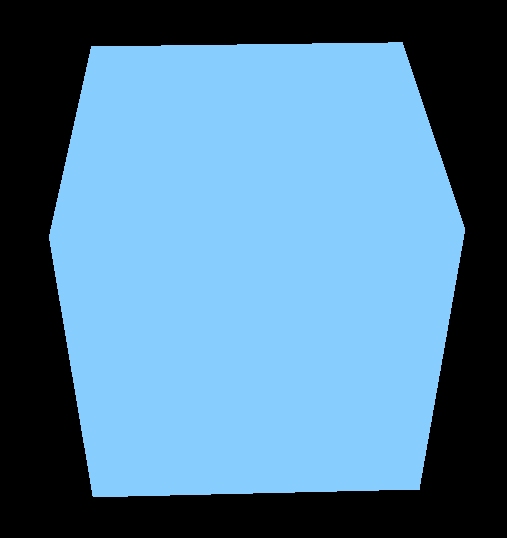
\includegraphics[scale=0.45]{caixaP} 
\caption{\label{fig:controller}Exemplo de uma caixa com divisões}
\end{figure} \begin{figure}[H]
\centering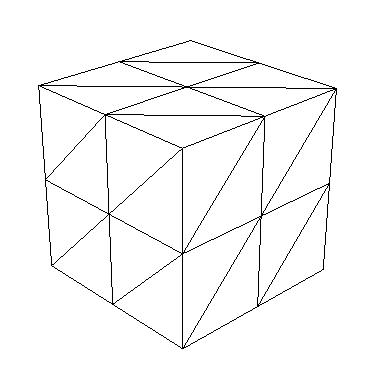
\includegraphics[scale=0.4]{caixaT} 
\caption{\label{fig:controller}Exemplo de uma caixa com divisões com a representação dos triângulos}
\end{figure}
\newpage
\section{Esfera}
O cálculo dos pontos de uma esfera necessita de 3 parâmetros: raio, slices que correspondem às divisões na vertical ao longo da esfera e stacks que correspondem às divisões na horizontal ao longo da esfera
Quanto maior o número de slices e stacks, maior será o número de pontos a determinar, ou seja, melhor será a precisão da esfera. Sabemos que:
\begin{itemize}
\item A intersecção entre uma slice e uma stack origina 4 pontos
\item A distância entre cada um destes pontos ao centro é o raio
\item Podemos ter um vetor para cada ponto, e esse vetor tem dois ângulos, um relativo ao eixo dos $yy$(\textbeta) e outro relativo ao eixo dos $zz$(\textalpha). Em vez de termos relativo ao eixo dos zz, poderíamos ter relativo ao eixo dos xx
\item O ângulo \textalpha $\in$ [0; 2$\pi$] e depende do número de slices
\item O ângulo \textbeta $\in$ [0; $\pi$], e depende do número de stacks
\item Temos um \textDelta\textalpha \ que será calculado através $\frac{2\times\pi}{slices}$
\item Temos um \textDelta\textbeta \ que será calculado através $\frac{\pi}{stacks}$
\end{itemize}
\begin{figure}[H]
\centering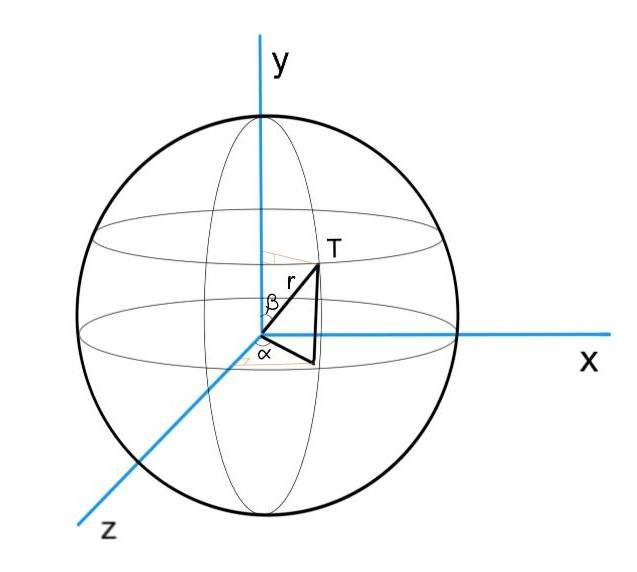
\includegraphics[scale=0.50]{esfera} 
\caption{\label{fig:controller}Representação de um ponto T na superfície de uma esfera e os respetivos ângulos}
\end{figure}
Após a nossa representação da esfera, facilmente conseguimos retirar as equações para transformar as coordenadas polares em cartesianas do ponto T:
\begin{center}
$x = r \times \sin(\beta) \times \sin(\alpha)$

$y = r \times \cos(\beta)$

$z = r \times \sin(\beta) \times \cos(\alpha)$ 
\end{center}
\begin{figure}[H]
\centering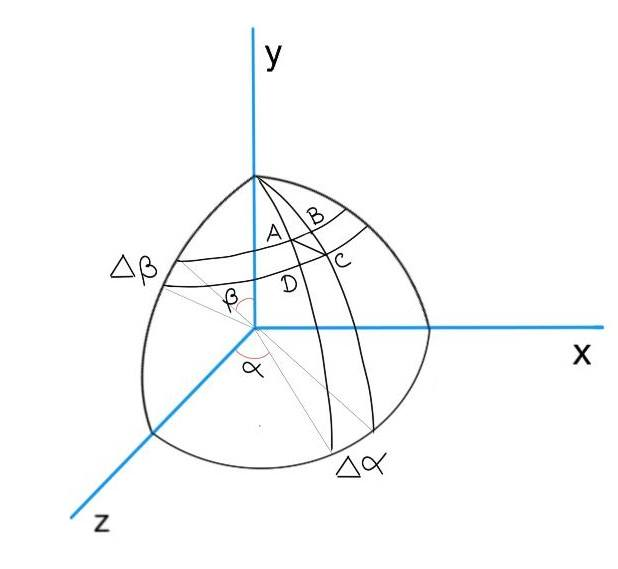
\includegraphics[scale=0.50]{esfera2} 
\caption{\label{fig:controller}Representação dos 4 pontos de uma interseção}
\end{figure}
Na figura acima apresentada demonstramos um exemplo de uma interseção entre slices e stacks em que geramos os pontos $A,B,C$ e $D$.
Estes pontos servirão para calcular os vértices correspondentes aos triângulos $ABC$ e $ACD$. Por último falta-nos determinar, os ângulos correspondentes
aos pontos $B, C$ e $D$.\newline
\begin{center}
\begin{tabular}{||c c c||} 
\hline
Ponto & \textalpha & \textbeta \\ [0.5ex] 
\hline\hline
B & \textalpha + \textDelta\textalpha & \textbeta\\ 
\hline
C & \textalpha + \textDelta\textalpha & \textbeta + \textDelta\textbeta \\
\hline
D & \textalpha & \textbeta + \textDelta\textbeta\\ [1ex] 
    \hline
\end{tabular}
\end{center}
\textbf{Para cada stack i} $\{$\newline
\par $\beta = i \times \Delta\beta$ \newline
\par \textbf{Para cada slice j} $\{$ \newline
\par $\alpha = j \times \Delta\alpha$ \newline\newline
\par\textit{\textbf{Ponto A}} \newline
\par$x = r\times\sin(\beta)\times\sin(\alpha)$ \newline
\par$y = r\times\cos(\beta)$ \newline
\par$z = r\times\sin(\beta)\times\cos(\alpha)$ \newline\newline
\par\textit{\textbf{Ponto B}} \newline
\par$x = r\times\sin(\beta)\times\sin(\alpha + \Delta\alpha)$ \newline
\par$y = r\times\cos(\beta)$ \newline
\par$z = r\times\sin(\beta)\times\cos(\alpha + \Delta\alpha)$ \newline\newline
\par\textit{\textbf{Ponto C}} \newline
\par$x = r\times\sin(\beta + \Delta\beta)\times\sin(\alpha + \Delta\alpha)$ \newline
\par$y = r\times\cos(\beta + \Delta\beta)$ \newline
\par$z = r\times\sin(\beta + \Delta\beta)\times\cos(\alpha + \Delta\alpha)$ \newline\newline
\par\textit{\textbf{Ponto D}} \newline
\par$x = r\times\sin(\beta + \Delta\beta)\times\sin(\alpha)$ \newline
\par$y = r\times\cos(\beta + \Delta\beta)$ \newline
\par$z = r\times\sin(\beta + \Delta\beta)\times\cos(\alpha)$ \newline
\par $\}$ \newline
$\}$
\newpage
Exemplo: \textit{sphere 4 100 100}
\begin{figure}[H]
\centering
\includegraphics[scale=0.35]{esferaP} 
\caption{\label{fig:controller}Exemplo de uma esfera}
\end{figure} \begin{figure}[H]
\centering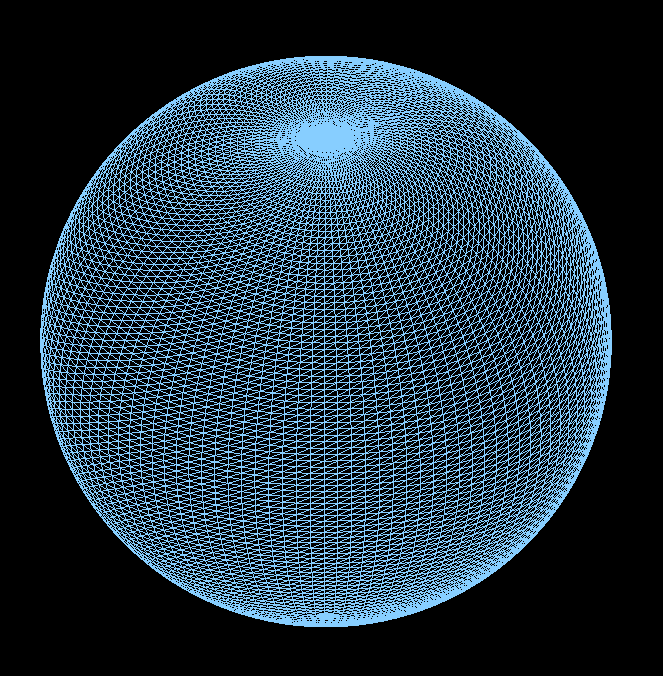
\includegraphics[scale=0.35]{esferaT} 
\caption{\label{fig:controller}Exemplo de uma esfera com a representação dos triângulos}
\end{figure}
\newpage
\section{Cone}
Para calcular os pontos que constituem um cone é necessário os seguintes parâmetros: raio, altura, slices e stacks.
Dado não se tratar de uma primitiva regular, foi preciso optar por uma prática recorrente Divide and Conquer, 
resolvendo inicialmente a base do nosso cone, e só após isso a superfície lateral. Sabemos que a base vai ser constituída por vários triângulos
unidos ao centro, cada um com o seu ângulo $\alpha$ respetivo. Para a geração dos pontos que irão representar a base do cone, foi necessário recorrer ao 
sistema de coordenadas polares, para transformar em coordenadas cartesianas. Apresentamos então as fórmulas para o cálculo da base:\newline\newline
$x = r\times\sin(\alpha)$\newline\newline
$z=r\times\cos(\alpha)$\newline\newline
$\Delta\alpha = \frac{2\times\pi}{slices}$\newline
\begin{figure}[H]
\centering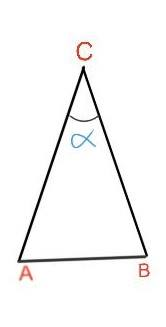
\includegraphics[scale=0.50]{triangulo} 
\caption{\label{fig:controller}Imagem ilustrativa de um triângulo da base do cone}
\end{figure}
\textbf{Para cada slice i} $\{$\newline
\par $\alpha = i \times \Delta\alpha$ \newline\newline
\par\textit{\textbf{Ponto A}} \newline
\par$x = r\times\sin(\alpha)$\newline
\par$y = 0$ \newline
\par$z = r\times\cos(\alpha)$ \newline\newline
\par\textit{\textbf{Ponto B}} \newline
\par$x = r\times\sin(\alpha + \Delta\alpha)$ \newline
\par$y = 0$ \newline
\par$z = r\times\cos(\alpha + \Delta\alpha)$  \newline\newline
\par\textit{\textbf{Ponto C}} \newline
\par$x = 0$\newline
\par$y = 0$ \newline
\par$z = 0$ \newline
$\}$
\newline\newline
Os ciclos que foram implementados posteriormente para a geração dos vértices da superfície lateral, seguem a mesma lógica da esfera,
a intersecção entre uma slice e uma stack resulta em quatro pontos. Porém existe a necessidade de definir um novo raio e aumentar a respectiva altura do modelo a cada
camada ao longo da iteração. Além das fórmulas já declaradas acima que também iremos precisar para a superfície, temos mais esta equação:\newline\newline
\par$\Delta y = \frac{altura}{stacks}$\newline
\begin{figure}[H]
\centering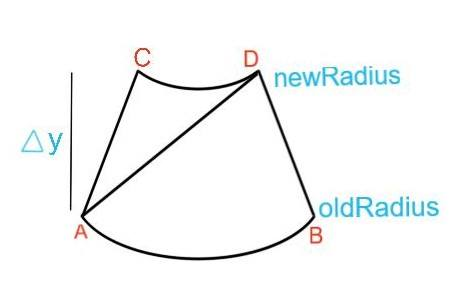
\includegraphics[scale=0.50]{coneAux} 
\caption{\label{fig:controller}Imagem ilustrativa de uma intersecção na superfície lateral do cone}
\end{figure}
\textbf{Para cada stack i} $\{$\newline
\par $y = i \times \Delta y$ \newline
\par $newR = \frac{r}{altura} \times (altura - ((i+1) \times \Delta y))$ \newline
\par \textbf{Para cada slice j} $\{$ \newline
\par $\alpha = j \times \Delta\alpha$ \newline\newline
\par\textit{\textbf{Ponto A}} \newline
\par$x = oldR\times\sin(\alpha)$ \newline
\par$y = y$ \newline
\par$z = oldR\times\cos(\alpha)$ \newline\newline
\par\textit{\textbf{Ponto B}} \newline
\par$x = oldR\times\sin(\alpha + \Delta\alpha)$ \newline
\par$y = y$ \newline
\par$z = oldR\times\cos(\alpha + \Delta\alpha)$ \newline\newline
\par\textit{\textbf{Ponto C}} \newline
\par$x = newR\times\sin(\alpha)$ \newline
\par$y = y + \Delta y$ \newline
\par$z = newR\times\cos(\alpha)$ \newline\newline
\par\textit{\textbf{Ponto D}} \newline
\par$x = newR\times\sin(\alpha + \Delta\alpha)$ \newline
\par$y = y + \Delta y$ \newline
\par$z = newR\times\cos(\alpha + \Delta\alpha)$ \newline\newline
\par $\}$ \newline\newline
$oldR = newR;$\newline\newline
$\}$
\newpage
Exemplo: \textit{cone 1 2 50 50}
\begin{figure}[H]
\centering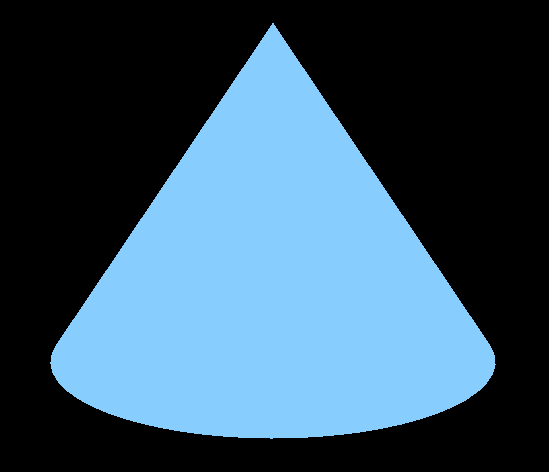
\includegraphics[scale=0.45]{coneP} 
\caption{\label{fig:controller}Exemplo de um cone}
\end{figure} \begin{figure}[H]
\centering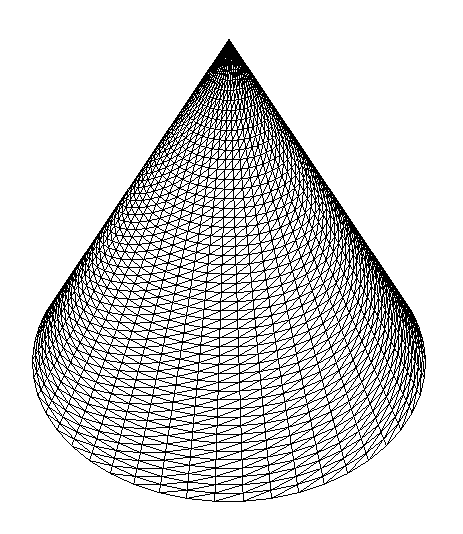
\includegraphics[scale=0.48]{coneT} 
\caption{\label{fig:controller}Exemplo de um cone com a representação dos triângulos}
\end{figure}
\newpage
\section{Motor}
A aplicação Engine tem como objetivo ler e interpretar um ficheiro de configuração XML, com recurso à biblioteca tinyXML2, que contém uma lista
com os ficheiros anteriormente criados pelo Gerador, e desenhar em OpenGL as figuras contidas nesse ficheiro.
\begin{center}
\fbox{\begin{minipage}{10em}
Engine.exe <xmlFile>
\end{minipage}}
\end{center}
\section{Extras}
Durante a realização do trabalho decidimos implementar algumas funcionalidades que por sua vez facilitaram a verificação dos resultados obtidos e permitiram uma melhor interação com os modelos produzidos pelo generator. 
\begin{itemize}
\item PolygonMode : Polígonos podem ser desenhados de forma preenchida,apenas com as linhas e contorno ou
somente os vértices. Um polígono tem dois lados (front e back), que podem ser renderizados diferentemente dependendo do lado que observador estiver a observar. Para tal utilizamos os seguintes comandos:
\textit{P, L e F}.
\item Zoom: Optou-se por implementar o zoom de modo a ser possível fazer aproximações da câmera sobre os diferentes modelos , para tal efeito utilizamos as seguintes teclas:\newline
\textit{Zoom in :  X}\newline
\textit{Zoom out :  Z}
\item Rotações e Translações : Durante a resolução dos problemas propostos, sentimos a necessidade de
interagir com os modelos através de rotações e translações de forma a podermos concluir com toda a
certeza que todas as faces/triângulos do modelo eram desenhadas. Para tal efeito utilizamos as seguintes teclas:\newline
\textit{Rotações : Q, E e as setas}\newline
\textit{Translações: W, S, A e D}
\item ChangeModel: Para uma troca entre os diferentes modelos optou-se por realizar
a função changeModel,para efectuar as mudanças utilizamos as seguintes teclas: \textit{N e M}.
\end{itemize}
\newpage
\section{Conclusão}
Com a elaboração desta fase do projeto aprofundamos os nossos conhecimentos em relação à ferramenta usada OpenGL, assim como exploramos a linguagem C++.
Todos os requisitos propostos nesta fase foram cumpridos, estando todos funcionais, e ainda foram implementados algumas funcionalidades extra no motor para
verificar a correta construção das primitivas. 
\end{document}